\documentclass{beamer}
% This is the file main.tex
\usetheme{Dresden}
\usepackage{tikz}
\setbeamertemplate{navigation symbols}{}
\setbeamertemplate{mini frames}{}
\renewcommand*{\slideentry}[6]{}
\addtobeamertemplate{navigation symbols}{}{%
    \usebeamerfont{footline}%
    \usebeamercolor[fg]{footline}%
    \hspace{1em}%
    \ifnum\value{framenumber}>0
    {\insertframenumber/\inserttotalframenumber}
    \fi
}
\setbeamercolor{structure}{fg=MyPurple}
\definecolor{MyPurple}{RGB}{105,18,83}
\usepackage{graphicx}
\usepackage{amsmath}
\usepackage[euler]{textgreek}
\usepackage{adjustbox}
\usepackage{booktabs}
\usepackage{multirow}
\usepackage{multirow, xspace, amsmath}
\usepackage{pdfpages}
\usepackage{fancybox}
\usepackage{stackengine}
\usepackage{cancel}
%\usepackage{geometry}
%\geometry{
% a4paper,
% total={170mm,257mm},
% left=20mm,
% top=20mm,
% }
\newcommand*{\ttbar}{\ensuremath{t\bar{t}}\xspace}
\newcommand*{\mbb}{\ensuremath{\text{m}_{bb}}\xspace}
\newcommand*{\dsig}{\ensuremath{|\sigma_{d_{0}}|}\xspace} 
\newcommand*{\met}{\ensuremath{\cancel{E_{T}}}\xspace}
\newcommand{\backupbegin}{
   \newcounter{framenumberappendix}
   \setcounter{framenumberappendix}{\value{framenumber}}
}
\newcommand{\backupend}{
   \addtocounter{framenumberappendix}{-\value{framenumber}}
   \addtocounter{framenumber}{\value{framenumberappendix}} 
}
\newcommand\tab[1][1cm]{\hspace*{#1}}

\newcommand*{\header}[1]{\fontsize{16}{8}\selectfont \textbf{{\color{MyPurple}{#1}}}}

\usepackage{tikz}
\usepackage[compat=1.1.0]{tikz-feynman}


\title{Search For Double Higgs Production in the $b\bar{b}WW^{*}$ Channel}
\subtitle{}
\author[John C.S. Myers]{John C.S. Myers}
\institute[University of Oregon]{ University of Oregon}
\date{\today}


\begin{document}
%\begin{frame}[noframenumbering]
%\titlepage
%\end{frame}
{ \setbeamertemplate{footline}{} \begin{frame}[noframenumbering] \titlepage \end{frame} }
%%Start with general into and then briefly on trigger
%% highlight talks and being public face
%%
%%need to think of transiton into HHbbWW
%%
%%HHbbWW paper analysis-->leptons inside jets-->how to use ANL computing


\begin{frame}
\begin{center}
\header{Overview}
\end{center}
\begin{itemize}
%\small
\item The Standard Model and Higgs Physics
\item BSM Double Higgs Production
\item The LHC and ATLAS
\item $HH\rightarrow{}b\bar{b}WW^{*}$ Analysis
\item Improvements to the Analysis
\item Conclusion and Outlook
\end{itemize}
\end{frame}

\begin{frame}
\begin{center}
\header{The Standard Model}
\end{center}
\begin{columns}
\begin{column}{0.5\textwidth}
\begin{itemize}
\item Describes matter (fermions) and force carriers (gauge bosons)
\item Very successful model
\item The discovery of the final piece (Higgs Boson) announced in 2012
\end{itemize}
\end{column}
\begin{column}{0.5\textwidth}
\includegraphics[width=1\textwidth]{figures/Standard_Model_of_Elementary_Particles}
\end{column}
\end{columns}
\end{frame}

\begin{frame}
\begin{center}
\header{Higgs Mechanism}
\end{center}
\begin{columns}
\begin{column}{0.5\textwidth}
\color{MyPurple}{Scalar Boson}\color{black}
\begin{center}
$\phi = \frac{1}{\sqrt{2}}\binom{\phi^+}{\phi^0}$\\~\\
\huge$\Downarrow$ \normalsize EWSB \huge$\Downarrow$ \normalsize\\~\\
$\phi_0 = \frac{1}{\sqrt{2}}\binom{0}{v};\ \phi(x) = \frac{1}{\sqrt{2}}\binom{0}{v + h(x)}$\\~\\
Coupling to Gauge Bosons gives $W^{\pm},\ Z,\ A(\gamma)$\\~\\
$M_W^2 = \frac{1}{4}g^2v^2$\\~\\
\vspace{-0.3cm}$M_Z^2 = \frac{1}{4}(g^2 + g'^{2})v^2$\\~\\
\vspace{-0.3cm}$M_A^2 = 0$
\end{center}
\end{column}
\begin{column}{0.5\textwidth}
\begin{center}
\includegraphics[width=0.75\textwidth]{figures/higgspotential}\\
\includegraphics[width=0.6\textwidth]{figures/Higgs_mech}
\end{center}
\end{column}
\end{columns}
\end{frame}

\begin{frame}
\begin{center}
\header{Higgs Self-Coupling}
\end{center}
\begin{columns}
\begin{column}{0.5\textwidth}
\includegraphics[width=1\textwidth]{figures/higgspotential}
\end{column}
\begin{column}{0.5\textwidth}
\color{MyPurple}{Higgs Potential}\color{black}
\begin{center}
$V = \mu^2|\Phi^{\dagger}\Phi| + \lambda(|\Phi^{\dagger}\Phi|)^2$\\~\\
Expand self-coupling around $v$\\~\\
$V_\mathrm{self-coupling} \supset{} \lambda{}v\Phi^3 + \frac{\lambda}{4}\Phi^4$\\~\\
Tri-linear Higgs coupling strength $\lambda_{HHH}\equiv{}\lambda v$
\end{center}
\end{column}
\end{columns}
\end{frame}

\begin{frame}
\begin{center}
\header{Higgs Self-Coupling}
\end{center}
\begin{columns}
\begin{column}{0.5\textwidth}
\begin{center}
\includegraphics[width=0.75\textwidth]{figures/sm_fey}\\~\\
SM Theory cross section:\\
\small$\sigma_{\mathrm{HH}} \approx 33.53\mathrm{fb}$
\end{center}
\end{column}
\begin{column}{0.5\textwidth}
Two Dominant production modes at the LHC\\~\\
Interfere destructively to give small theoretical cross section\\
\begin{center}
\includegraphics[width=0.75\textwidth]{figures/SM_continuum}
\end{center}
\end{column}
\end{columns}
\end{frame}


\begin{frame}
\begin{center}
\header{Motivation}
\end{center}
\begin{columns}
\begin{column}{0.5\textwidth}
\textcolor{MyPurple}{Resonant Double Higgs production}\\
\begin{itemize}
\item A New process could decay to $HH$
\item E.g. Real Higgs Singlet Extension
\begin{itemize}
\item Couples to SM Higgs
\item Large enhancement to HH production rate
\begin{itemize}
\item Up to 30 times SM 
\end{itemize}
\end{itemize}
\end{itemize}
\begin{center}
\color{MyPurple}{By measuring the HH production rate, we can search for resonant production}
\end{center}
\end{column}
\begin{column}{0.5\textwidth}
\begin{figure}[h]
\footnotesize
\begin{center}
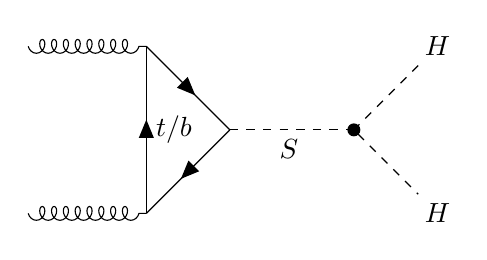
\begin{tikzpicture}
\begin{feynman}
\vertex (i1);
\vertex [right = of i1] (t1);
\vertex [dot][below right =of t1] (t3);
\vertex [below left= of t3] (t2);
\vertex [left = of t2] (i2);
\vertex [right =of t3][dot](h){};
\vertex [above right = of h] (f1){\(H\)};
\vertex [below right = of h] (f2){\(H\)};
\diagram* {
(i1) -- [gluon] (t1),
(i2) -- [gluon] (t2),
(t1) -- [fermion](t3) -- [fermion] (t2) -- [fermion,edge label'=\(t/b\)](t1),
(t3) -- [scalar,edge label'=\(S\)] (h),
(f1) -- [scalar] (h) -- [scalar](f2)
};
\end{feynman}
\end{tikzpicture}\\
\includegraphics[width=0.75\textwidth]{figures/ian6}
\end{center}
\end{figure}
\end{column}
\end{columns}
\end{frame}

%\begin{frame}
%\begin{center}
%\header{}
%\end{center}
%\end{frame}

\begin{frame}
\begin{center}
\header{$\mathbf{HH\rightarrow{}b\bar{b}WW^{*}}$ Semi-Leptonic Channel}
\end{center}
\vspace{-0.6cm}
\begin{columns}
\begin{column}{0.5\textwidth}
\begin{itemize}
\item $b\bar{b}WW^*$ has the second highest BR behind $b\bar{b}b\bar{b}$
\item W can decay leptonically or hadronically:
\begin{itemize}
\footnotesize
\item Charged lepton + neutrino or 
\item quark + anti-quark
\end{itemize}
\item Choose $bbl\nu{}qq$ final state 
\begin{itemize}
\footnotesize
\item Lepton helps against QCD
\item Neutrino makes reco. more challenging
\end{itemize}
\end{itemize}
\end{column}
\begin{column}{0.5\textwidth}
\begin{center}
\includegraphics[width=01.2\textwidth]{figures/pie_chart}
%\includegraphics[width=0.75\textwidth]{figures/comb_limit}
\end{center}
\end{column}
\end{columns}
\end{frame}

\begin{frame}
\begin{center}
\header{${\mathbf{bbl\boldsymbol{\nu{}}qq}}$ Final State}
\end{center}
\begin{columns}
\begin{column}{0.5\textwidth}
\begin{itemize}
\item electron or muon
\item 2 b quarks
\item 2 light flavor quarks
\item neutrino
\end{itemize}
\end{column}
\begin{column}{0.5\textwidth}
\begin{center}
\includegraphics[width=1\textwidth]{figures/res_prod}
\end{center}
\end{column}
\end{columns}
\end{frame}

\begin{frame}
\begin{center}
\header{Jets}
\end{center}
\begin{itemize}
\item Quarks hadronize before they interact with the detector
\item Gives sprays of energy deposits
\item Energy deposits grouped together into ``Jets" by algorithms
\end{itemize}
\begin{center}
\includegraphics[height=0.5\textheight]{figures/antikt}
\end{center}
\end{frame}

\begin{frame}
\begin{center}
\header{Neutrinos}
\end{center}
\begin{itemize}
\item Neutrinos do not interact with detector
\item Have transverse (perpendicular to beam line) information from \met
\item Need another piece to fully reconstruct 4-momentum
\begin{itemize}
\item This analysis used Higgs mass
\end{itemize}
\end{itemize}
\begin{center}
\includegraphics[height=0.5\textheight]{figures/met}
\end{center}
\end{frame}

\begin{frame}
\begin{center}
\header{${\mathbf{bbl\boldsymbol{\nu{}}qq}}$ Final State}
\end{center}
\begin{columns}
\begin{column}{0.5\textwidth}
\begin{itemize}
\item electron or muon
\item 2 light jets
\item 2 b-jets
\item \met
\end{itemize}
\end{column}
\begin{column}{0.5\textwidth}
\begin{center}
\includegraphics[width=1\textwidth]{figures/res_prod}
\end{center}
\end{column}
\end{columns}
\end{frame}


\begin{frame}
\begin{center}
\header{Background}
\begin{columns}
\begin{column}{0.3\textwidth}
\color{MyPurple}{Major}
\begin{itemize}
\small
\item \ttbar
\item W+Jets
\item QCD multijet
\end{itemize}
Minor
\begin{itemize}
\small
\item Z+Jets
\item Single Top
\item Diboson
\end{itemize}
\end{column}
\begin{column}{0.7\textwidth}
\begin{center}
\color{MyPurple}{\ttbar vs signal}
\end{center}
\begin{center}
\includegraphics[width=0.45\textwidth]{figures/cartoon_tt}
\includegraphics[width=0.45\textwidth]{figures/cartoon_hh_crop}
\end{center}
\end{column}
\end{columns}
\end{center}
\end{frame}

\begin{frame}
\begin{center}
\header{The Large Hadron Collider}
\end{center}
\begin{columns}
\begin{column}{0.6\textwidth}
\includegraphics[width=1\textwidth]{figures/LHC}
\end{column}
\begin{column}{0.4\textwidth}
\includegraphics[width=1\textwidth]{figures/dataset}
\end{column}
\end{columns}
\begin{columns}
\begin{column}{0.5\textwidth}
\begin{itemize}
\small
\item 13 TeV CoM Proton-Proton Collider
\item 27 km Circumference under the French-Swiss border
\end{itemize}
\end{column}
\begin{column}{0.5\textwidth}
\begin{itemize}
\small
\item 4 primary interaction points, each with a dedicated detector
\item Run 2 delivered 158 fb\textsuperscript{-1}
\end{itemize}
\end{column}
\end{columns}
\end{frame}

\begin{frame}
\begin{center}
\header{The ATLAS Detector}
\end{center}
\begin{center}
\includegraphics[width=0.8\textwidth]{figures/ATLAS_det}
\end{center}
%\begin{columns}
%\begin{column}{0.5\textwidth}
%\begin{itemize}
%\item General purpose detector
%\end{itemize}
%\end{column}
%\begin{column}{0.5\textwidth}
%\begin{itemize}
%\item Up to 3.9 T Toroid
%\end{itemize}
%\end{column}
%\end{columns}
\end{frame}

\begin{frame}
\begin{center}
\header{Particles in the Detector}
\end{center}
\begin{center}
\includegraphics[width=0.75\textwidth]{figures/layers}
\end{center}
\end{frame}

\begin{frame}
\begin{center}
\header{ATLAS Trigger}
\end{center}
\begin{columns}
\begin{column}{0.5\textwidth}
\begin{itemize}
\item LHC has 40 MHz Collision Rate
\begin{itemize}
\item $\sim$64 TB/s 
\end{itemize}
\item 2 Level Trigger System
\begin{itemize}
\item Level-1 Trigger (L1)
\item High Level Trigger (HLT)
\end{itemize}
\item Reduces rate from 40MHz to $\sim$1 kHz ($\sim$2 GB/s)
\end{itemize}
\end{column}
\begin{column}{0.5\textwidth}
\includegraphics[width=1\textwidth]{figures/run2TDAQ}
\end{column}
\end{columns}
\end{frame}

\begin{frame}
\begin{center}
\header{$\mathbf{HH\rightarrow{}b\bar{b}WW^*}$ Analysis}
\end{center}
2 Separate Analyses Presented:
\begin{itemize}
\item 2015-2016, $36.1 \text{ fb}^{-1}$ Analysis
\begin{itemize}
\item \href{https://link.springer.com/article/10.1007/JHEP04(2019)092}{JHEP04(2019)092}
\end{itemize}
\item Improvements for full Run 2 analysis
\end{itemize}
\end{frame}

\begin{frame}
\begin{center}
\header{Resolved Event Selection}
\end{center}
\begin{center}
\includegraphics[width=1\textwidth]{figures/resolvedv2}
\end{center}
\color{MyPurple}{\textbf{Designed to target SM production and $\mathbf{m_S < 1300}$ GeV}}
\end{frame}

\begin{frame}
\begin{center}
\header{Boosted Event Selection}
\end{center}
\begin{center}
\includegraphics[width=1\textwidth]{figures/boostedv2}
\end{center}
\color{MyPurple}{\textbf{Designed to target $\mathbf{m_S > 1300}$ GeV}}
\end{frame}

\begin{frame}
\begin{center}
\header{Signal Region}
\end{center}
\begin{columns}
\begin{column}{0.5\textwidth}
\begin{center}
\color{MyPurple}{Resolved}
\begin{itemize}
\item $\met{} > 25$ GeV
\item Large $p_T^{bb}$
\item Large $p_T^{WW}$
\item $m_{bb}\sim{}m_H$
\item $m_{HH}\sim{}m_{S}$
\end{itemize}
\end{center}
\end{column}
\begin{column}{0.5\textwidth}
\begin{center}
\vspace{-1.4cm}\color{MyPurple}{Boosted}
\end{center}
\begin{itemize}
\item $\met{} > 50$ GeV
\item $m_\mathrm{Large-R\ jet}\sim{}m_H$
\end{itemize}
\end{column}
\end{columns}
\end{frame}

\begin{frame}
\begin{center}
\header{Resolved Background Determination}
\end{center}
\begin{columns}
\begin{column}{0.5\textwidth}
\color{MyPurple}{\ttbar}
\begin{itemize}
\footnotesize
\item Normalized in $m_{bb}$ CR
\begin{itemize}
\scriptsize
\item Boosted \ttbar VR
\end{itemize}
\end{itemize}
\end{column}
\begin{column}{0.5\textwidth}
\color{MyPurple}{Other MC Bkg.}
\begin{itemize}
\footnotesize
\item Modeled using MC and normalized to SM XSec
\end{itemize}
\end{column}
\end{columns}
\begin{center}
\color{MyPurple}{QCD multi-jet background}
\end{center}
\begin{columns}
\begin{column}{0.5\textwidth}
\begin{itemize}
\vspace{-0.5cm}
\footnotesize
\item ABCD data driven estimate
\begin{itemize}
\item $N_A = F N_C N_B / N_D$
\item $F$ is a correction factor determined earlier in the cutflow
\item Boosted uses $\met>50\text{ GeV}$
\begin{itemize}
\scriptsize
\item Takes shape from 1 b-tag C Region
\end{itemize}
\end{itemize}
\end{itemize}
\end{column}
\begin{column}{0.5\textwidth}
\includegraphics[width=0.9\textwidth]{figures/abcdExample_met_vs_d0sigBL20}
\end{column}
\end{columns}
\end{frame}

\begin{frame}
\begin{center}
\header{Background Shape Check}
\end{center}
\begin{center}
\includegraphics[width=0.8\textwidth]{figures/C_mBBcr_reOpt2000_bbpt350_wlepmtben_regionA_met25d020-eps-converted-to}
\end{center}
\small
$m_T = \sqrt{2p_T^l\met\times{}(1-\cos{\Delta{\phi}})}$
\end{frame}

\begin{frame}
\begin{center}
\header{Resonant Production Signal Region}
\end{center}
\begin{center}
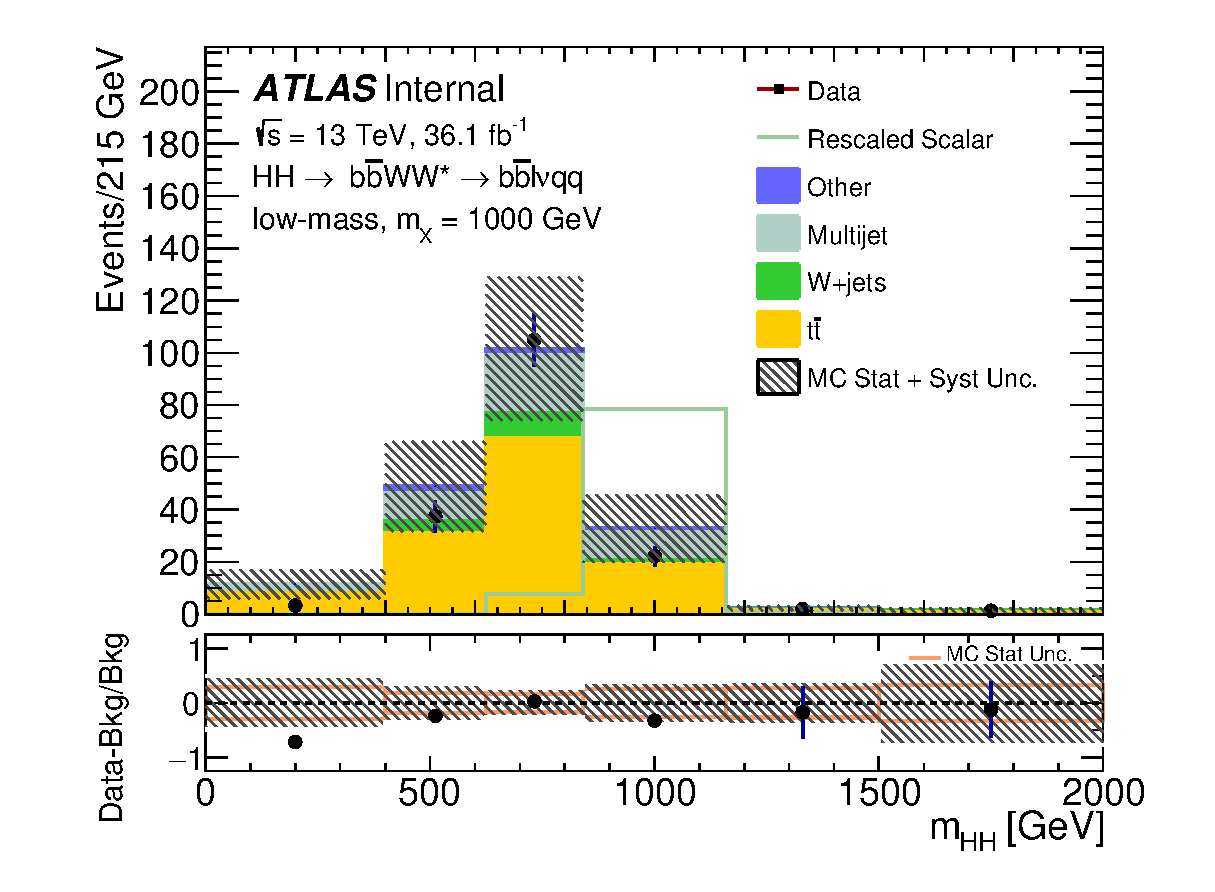
\includegraphics[width=0.8\textwidth]{figures/C_reOpt700_mww_bbpt210_wwpt250_mbb_hhMass_regionA_met25d020}
\end{center}
\end{frame}

\begin{frame}
\begin{center}
\header{Standard Model Results}
\end{center}
\begin{center}
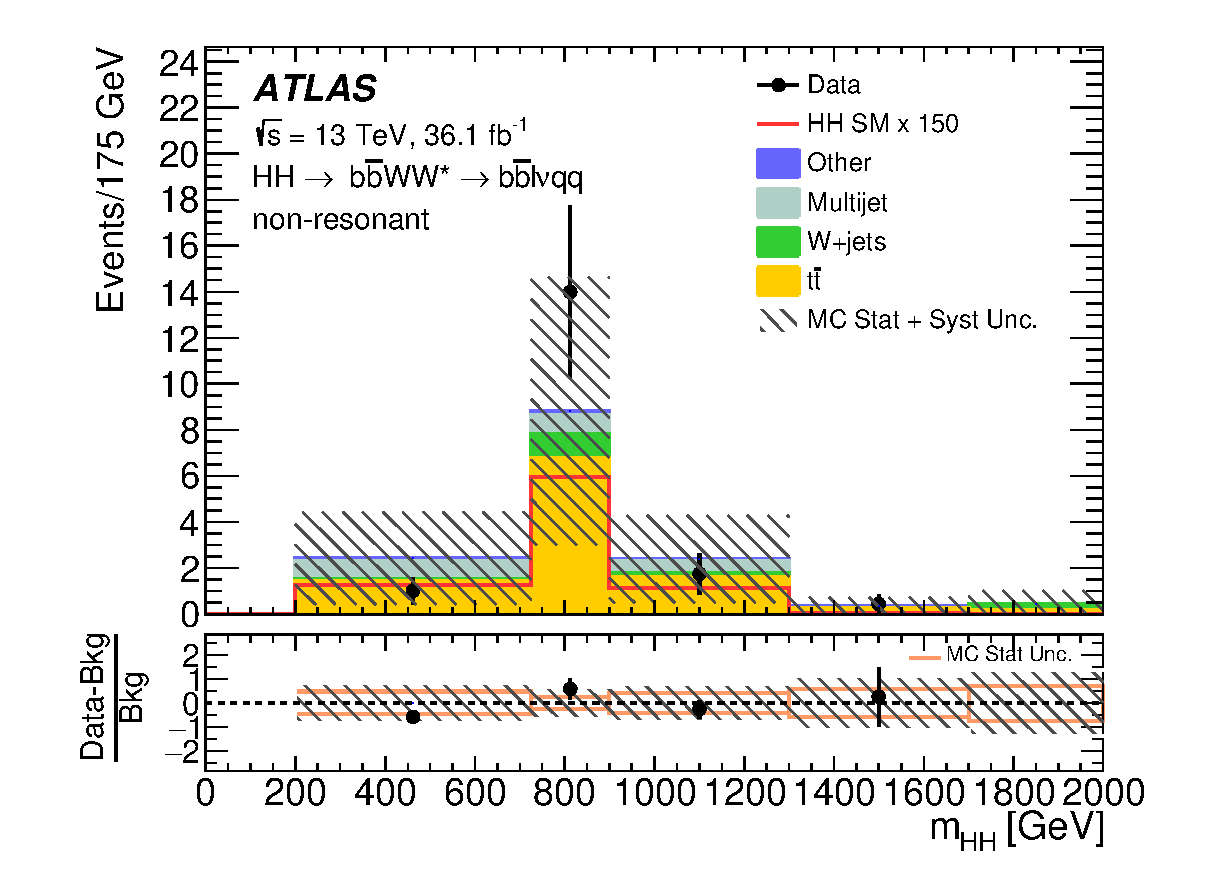
\includegraphics[width=0.7\textwidth]{figures/C_reOptNonRes_mww_bbpt210_bbpt300_wwpt250_mbb_hhMass_regionA_met25d020}
\end{center}
\color{MyPurple}{Production Cross Section 95\% CL}
\small
\vspace{-0.5cm}$\sigma(pp\rightarrow{}HH)B(HH\rightarrow{}b\bar{b}WW^*) < 300^{+100}_{-80} \times{} SM$
\end{frame}

\begin{frame}
\begin{center}
\header{Combined Resonant Production Limit}
\end{center}
\begin{center}
\includegraphics[width=0.65\textwidth]{figures/limit_2016_reOpt_HiggsApproved_Scalar_Paper_Combined_20190312_01}
\end{center}
\end{frame}

\begin{frame}
\begin{center}
\header{Motivation}
\end{center}
\vspace{-0.5cm}
\begin{columns}
\begin{column}{0.5\textwidth}
\begin{itemize}
\footnotesize
\item $H\rightarrow{}WW^*$ becomes boosted around 1 TeV 
\item Quarks become too close together to use 0.4 jets
\item Overlap removal with leptons kill efficiency
\item A ``Fully-Boosted" selection recovers lost efficiency at high $m_S$
\end{itemize}
\end{column}
\begin{column}{0.5\textwidth}
\begin{center}
\includegraphics[width=0.75\textwidth]{figures/drminlq}
\end{center}
\end{column}
\end{columns}
\end{frame}

\begin{frame}
\begin{center}
\header{Fully Boosted Event Selection}
\end{center}
\begin{center}
\includegraphics[width=1\textwidth]{figures/fullboost}
\end{center}
\end{frame}

\begin{frame}
\begin{center}
\header{Signal Reconstruction}
\end{center}
\begin{columns}
\begin{column}{0.5\textwidth}
\includegraphics[width=01\textwidth]{figures/electron/mww_e}
\end{column}
\begin{column}{0.5\textwidth}
\includegraphics[width=01\textwidth]{figures/electron/mhh_e}
\end{column}
\end{columns}
\small \color{MyPurple}{Previous Analysis:}
\begin{itemize}
\scriptsize
\item $H\rightarrow{WW} = $ 1 lepton + 2 AntiKt, R = 0.4 jets + $\nu$
\end{itemize}
\end{frame}

\begin{frame}
\begin{center}
\header{Background Modeling}
\end{center}
\begin{columns}
\begin{column}{0.5\textwidth}
\begin{itemize}
\item Same procedure as boosted paper analysis
\item ABCD data driven technique for QCD
\item Slightly looser selection to increase statistics
\item Check shape in mBB validation region
\end{itemize}
\end{column}
\begin{column}{0.5\textwidth}
\includegraphics[width=1\textwidth]{figures/ABCD}
\end{column}
\end{columns}
\end{frame}

\begin{frame}
\begin{center}
\header{Background Shape Check}
\end{center}
\begin{center}
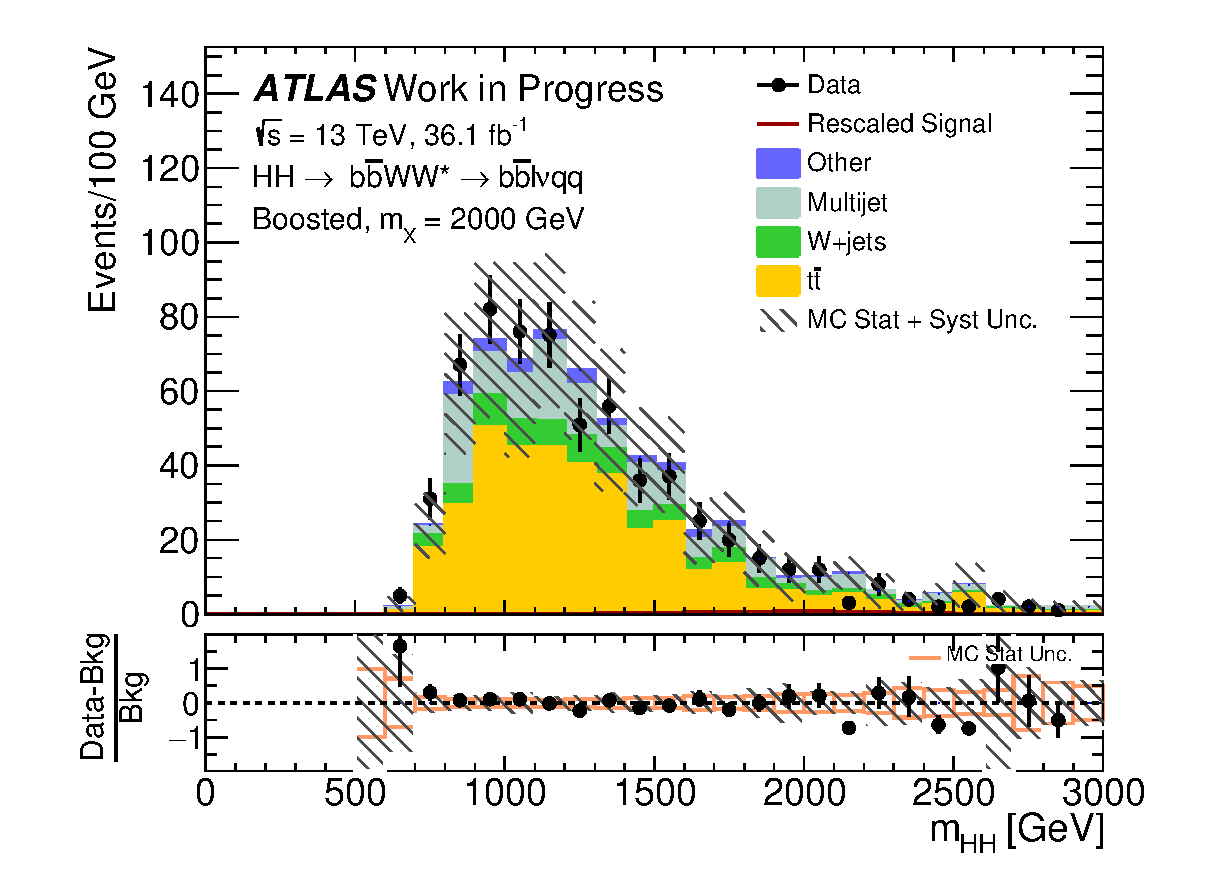
\includegraphics[width=0.9\textwidth]{figures/C_2tag_mbbcr_lepton_presel_met50_hhMassRebin1}
\end{center}
\end{frame}

\begin{frame}
\begin{center}
\header{Signal Region $\mathbf{m_{HH}}$}
\end{center}
\vspace{-0.2cm}
\begin{center}
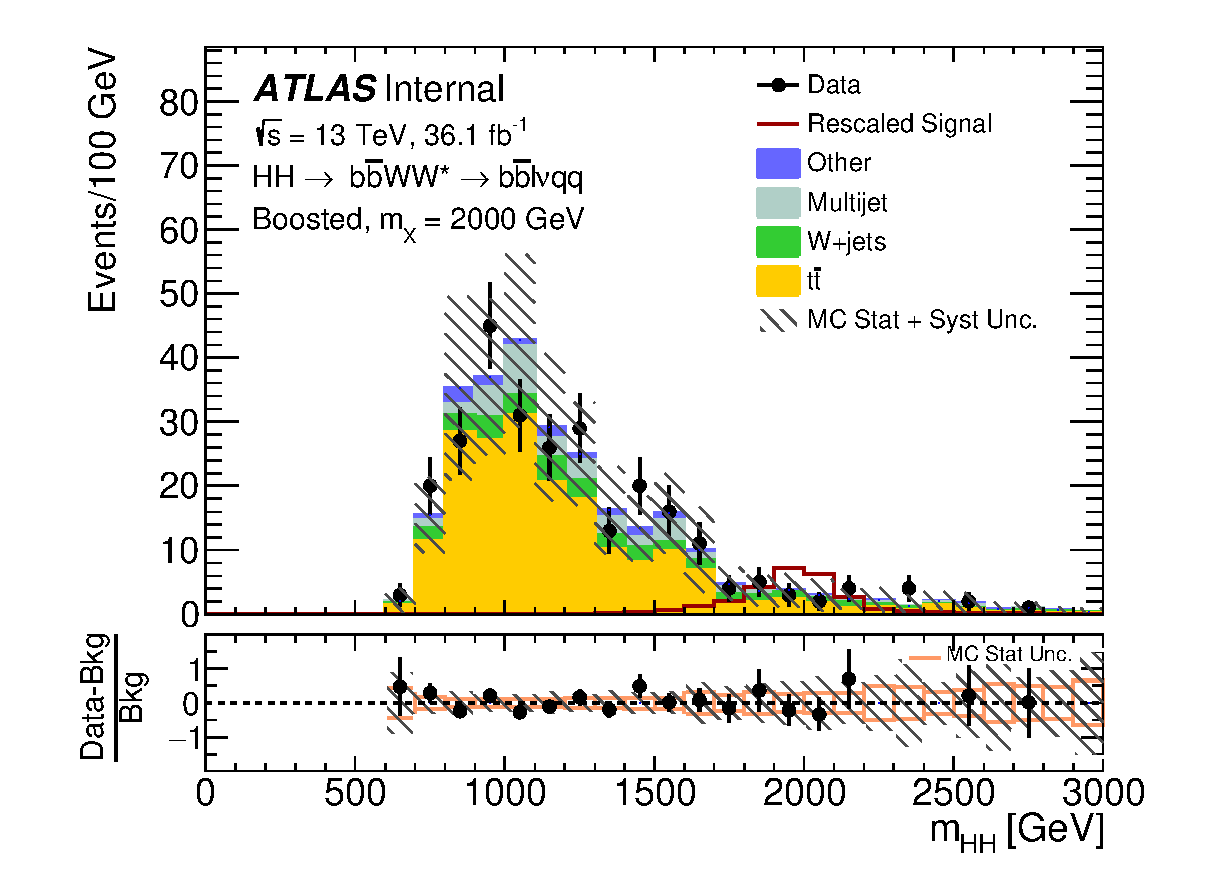
\includegraphics[width=0.9\textwidth]{figures/C_2tag_SR_lepton_presel_met50_hhMassRebin1}
\end{center}
\end{frame}

\begin{frame}
\begin{center}
\header{Results}
\end{center}
\begin{columns}
\begin{column}{0.5\textwidth}
\begin{center}
\color{MyPurple}{Published Analysis}
\includegraphics[width=01\textwidth]{figures/limit_2016_reOpt_HiggsApproved_Scalar_Paper_Combined_20190312_01_line}
\end{center}
\end{column}
\begin{column}{0.5\textwidth}
\begin{center}
\vspace{0.3cm}\color{MyPurple}{Improved Fully-Boosted Analysis}
\includegraphics[width=01\textwidth]{figures/Final_limits_line}
\end{center}
\end{column}
\end{columns}
\end{frame}

\begin{frame}
\begin{center}
\header{Conclusion}
\end{center}
\begin{itemize}
\item Set the first limits for $HH$ resonant production over 1 TeV
\item Developed analysis for SM $HH$ production in $b\bar{b}\rightarrow{}b\bar{b}l\nu{}qq$ channel
\begin{itemize}
\item Set limit of 300 X SM cross section
\end{itemize}
\item Improved the cross section upper limit for high resonant mass by $\sim$factor of 2
\end{itemize}
\end{frame}

\begin{frame}
\begin{center}
\header{Outlook}
\end{center}
\begin{itemize}
\item Move to Fatjet trigger
\begin{itemize}
\item Lepton ID requirement in derivation limits the high mass analysis
\end{itemize}
\item Neutrino reconstruction needs improved at high mass
\begin{itemize}
\item Use $H\rightarrow{}b\bar{b}$ information
\end{itemize}
\item ABCD estimate is limited by statistics
\begin{itemize}
\item Move to alternate QCD estimate like the Matrix Method
\end{itemize}
\end{itemize}
\end{frame}

\begin{frame}
\begin{center}
Thank you to my committee:\\
\textbf{Stephanie Majewski (Chair)}\\
\textbf{Tim Cohen}\\
\textbf{Hank Childs}\\
My Advisor: \textbf{Eric Torrence}\\
And a special thanks to Alison
\end{center}
\end{frame}

\begin{frame}
\begin{center}
\fontsize{16}{8}\selectfont \textbf{{\color{MyPurple}{Questions?}}}\\~\\
\end{center}
\end{frame}


\appendix
\backupbegin
\begin{frame}
\begin{center}
\fontsize{16}{8}\selectfont \textbf{{\color{MyPurple}{Backup}}}\\~\\
\end{center}
\end{frame}

\begin{frame}
\begin{center}
\header{Neutrino Reconstruction}
\end{center}
\begin{center}
$m_H^2 = (p^l + p^\nu + p^{i1} +p^{i2})^2$\\
Where $p^i$ is the 4-momentum of particle $i$\\
To find $p_z^\nu$, solve:\\
$p^\nu_E = E^\nu = \sqrt{p^2_T +p^2_z}\ ;p^\nu_x = p_T \cos{\phi}\ ;p^\nu_y = p_T \sin{\phi}\ $
\end{center}
\end{frame}

\begin{frame}
\begin{center}
\header{Resolved Signal Region}
\end{center}
\begin{table}
\begin{center}
\begin{tabular}{c|c|c|c|c}
 variable & \emph{Non-Res} & \emph{m500} & \emph{low-mass} & \emph{high-mass}\\
\hline
$\met$ (GeV)		&$> 25$&$>25$&$> 25$& $> 25$ \\
$m_{WW}$ (GeV) 	   		&$< 130$ &$< 130$ & $< 130$& no-cut\\
$p_{\rm T}^{bb}$ (GeV) 		&$> 300$& $> 210$&$> 210$&$> 350$\\
$p_{\rm T}^{WW}$ (GeV) 		&$> 250$&$> 150$&$> 250$&$> 250$ \\
$\Delta R_{WW}$  		&no-cut& no-cut&no-cut&$<1.5$\\
$m_{bb}$ (GeV)   		&105-135&105-135&105-135&105-135\\
\end{tabular}
\end{center}
\end{table}
\begin{table}
\begin{center}
\footnotesize
\begin{tabular}{c|c|c|c|c|c}
$m_{S}$ (GeV)      &   500   &   600   &   700   &   750   &   800 \\
$m_{HH}$  (GeV) & 480-530 & 560-640 & 625-775 & 660-840 & 695 - 905 \\ 
\hline 
$m_{S}$ (GeV)      &  900   &   1000  	   &  1100   	&  1200   		&   1300    \\
$m_{HH}$  (GeV) & 760-970	& 840-1160 & 925-1275	&1010-1390	&1095-1505  \\
\hline 
$m_{S}$ (GeV)      &   1400  		&  1500   		&  1600   		& 1800  		& 2000\\
$m_{HH}$  (GeV) &1250-1550	&1340-1660	&1430-1770	& 1750-2020 	& 1910-2170\\
\hline

\hline 
$m_{S}$ (GeV)      &   2250  		&  2500   		&  2750   		& 3000  		& \\
$m_{HH}$  (GeV) &2040-2460	&2330-2740	&2570-2950	& 2760-3210 	& \\
\end{tabular}
\end{center}
\end{table}
\end{frame}

\begin{frame}
\begin{center}
\header{mBBcr}
\end{center}
\begin{table}
\begin{center}
\tiny
\begin{tabular}{c|c|c|c|}
 variable &CR1 	& CR2 	& CR3 \\
\hline					
$m_{bb}$ (GeV)	& $m_{bb} < 100$ or $m_{bb} > 140$ & $m_{bb} < 100$ or $m_{bb} > 140$ & $m_{bb} < 100$ or $m_{bb} > 140$\\
$m_{WW}$ (GeV)   & $<130$ & $<130$& no-cut \\
$p_{\rm T}^{bb}$ (GeV) 	& $>300$ & $>210$&$>350$\\
\hline
\end{tabular}
\end{center}
\end{table}
\end{frame}

\begin{frame}
\begin{center}
\header{CR1}
\end{center}
\begin{table}
\tiny
\begin{tabular}{l|c|c|c|c}
\hline\hline
\multicolumn{5}{c}{\textbf{CR1}: \mbb Sideband}\\\hline\hline
Sample  	& mww 	& bbpt210 	& bbpt300 	& wwpt250 	  \\\hline
\ttbar 	& 23776.6 $\pm$ 87.2 	& 531.7 $\pm$ 13.1 	& 109.9 $\pm$ 5.9 	& 63.9 $\pm$ 4.6 \\\hline 
QCD 	& 13310.5 $\pm$ 500.3 	& 250.2 $\pm$ 30.6 	& 33.7 $\pm$ 4.1 	& 21.4 $\pm$ 2.6	\\\hline 
W+jets 	& 3938.9 $\pm$ 31.1 	& 124.7 $\pm$ 3.5 	& 29.3 $\pm$ 1.4 	& 17.1 $\pm$ 1.1 	\\\hline 
SingleTop 	& 1605.4 $\pm$ 18.0 	& 76.0 $\pm$ 3.8 	& 20.1 $\pm$ 2.0 	& 13.5 $\pm$ 1.7\\\hline 
Dibosons 	& 109.9 $\pm$ 2.7 	& 8.3 $\pm$ 0.8 	& 2.2 $\pm$ 0.4 	& 1.5 $\pm$ 0.4 	\\\hline 
Z+jets 	& 1107.6 $\pm$ 8.4 	& 27.1 $\pm$ 0.8 	& 6.7 $\pm$ 0.4 	& 2.4 $\pm$ 0.2 	\\\hline 
\hline
Background Sum 	& 43849.0$\pm$ 509.2 	& 1017.9$\pm$ 33.7 	& 201.9$\pm$ 7.6 	& 119.8$\pm$ 5.7 \\\hline 
\hline
XhhSM 	& 44.6 $\pm$ 2.2 	& 9.1 $\pm$ 0.7 	& 1.5 $\pm$ 0.2 	& 1.1 $\pm$ 0.1 	\\\hline 
Data 	& 43902.0 	& 1069.0 	& 206.0 	& 138.0 \\\hline 
\hline
\end{tabular}
\end{table}
\end{frame}

\begin{frame}
\begin{center}
\header{CR2 500}
\end{center}
\begin{table}
\tiny
\begin{tabular}{l|c|c|c|c}
\hline\hline
\multicolumn{5}{c}{\textbf{CR2}: \mbb Sideband}\\\hline\hline
Sample  	& mww 	& bbpt210 	& wwpt150 	& hh500  \\\hline
\ttbar 	& 23776.6 $\pm$ 87.2 	& 531.7 $\pm$ 13.1 	& 432.7 $\pm$ 11.8 	& 35.5 $\pm$ 3.2 		\\\hline 
QCD 	& 13310.5 $\pm$ 500.3 	& 250.2 $\pm$ 30.6 	& 206.3 $\pm$ 25.3 	& 16.9 $\pm$ 2.1 		\\\hline 
W+jets 	& 3938.9 $\pm$ 31.1 	& 124.7 $\pm$ 3.5 	& 105.9 $\pm$ 3.3 	& 4.9 $\pm$ 0.6 	\\\hline 
SingleTop 	& 1605.4 $\pm$ 18.0 	& 76.0 $\pm$ 3.8 	& 64.9 $\pm$ 3.5 	& 2.8 $\pm$ 0.6 	\\\hline 
Dibosons 	& 109.9 $\pm$ 2.7 	& 8.3 $\pm$ 0.8 	& 6.7 $\pm$ 0.8 	& 0.9 $\pm$ 0.2 	\\\hline 
Z+jets 	& 1107.6 $\pm$ 8.4 	& 27.1 $\pm$ 0.8 	& 19.0 $\pm$ 0.7 	& 1.5 $\pm$ 0.2 		\\\hline 
\hline
Background Sum 	& 43849.0$\pm$ 509.2 	& 1017.9$\pm$ 33.7 	& 835.5$\pm$ 28.3 	& 62.5$\pm$ 3.9	\\\hline 
\hline
Xhh500 	& 3.2 $\pm$ 0.1 	& 0.6 $\pm$ 0.1 	& 0.6 $\pm$ 0.1 	& 0.2 $\pm$ 0.1 	\\\hline 
Data 	& 43902.0 	& 1069.0 	& 898.0 	& 73.0 	\\\hline 
\end{tabular}
\end{table}
\end{frame}

\begin{frame}
\begin{center}
\header{CR2 700}
\end{center}
\begin{table}
\tiny
\begin{tabular}{l|c|c|c|c}
\hline\hline
\multicolumn{5}{c}{\textbf{CR2}: \mbb Sideband}\\\hline\hline
Sample  	& mww 	& bbpt210 	& wwpt250 	& hh700   \\\hline
\ttbar 	& 23776.6 $\pm$ 87.2 	& 531.7 $\pm$ 13.1 	& 175.6 $\pm$ 7.5 	& 49.9 $\pm$ 3.9 	\\\hline 
QCD 	& 13310.5 $\pm$ 500.3 	& 250.2 $\pm$ 30.6 	& 72.4 $\pm$ 8.9 	& 28.4 $\pm$ 3.5 		\\\hline 
W+jets 	& 3938.9 $\pm$ 31.1 	& 124.7 $\pm$ 3.5 	& 45.7 $\pm$ 2.1 	& 13.7 $\pm$ 1.4 	\\\hline 
SingleTop 	& 1605.4 $\pm$ 18.0 	& 76.0 $\pm$ 3.8 	& 28.4 $\pm$ 2.4 	& 6.9 $\pm$ 1.1 		\\\hline 
Diboson 	& 109.9 $\pm$ 2.7 	& 8.3 $\pm$ 0.8 	& 2.8 $\pm$ 0.5 	& 0.7 $\pm$ 0.2 		\\\hline 
Z+jets 	& 1107.6 $\pm$ 8.4 	& 27.1 $\pm$ 0.8 	& 5.8 $\pm$ 0.4 	& 2.0 $\pm$ 0.3 		\\\hline 
\hline
Background Sum 	& 43849.0$\pm$ 509.2 	& 1017.9$\pm$ 33.7 	& 330.7$\pm$ 12.1 	& 101.5$\pm$ 5.5 	\\\hline 
\hline
Xhh700 	& 4.2 $\pm$ 0.2 	& 2.2 $\pm$ 0.1 	& 1.5 $\pm$ 0.1 	& 1.0 $\pm$ 0.1 	\\\hline 
Data 	& 43902.0 	& 1069.0 	& 367.0 	& 124.0	\\\hline 
\end{tabular}
\end{table}
\end{frame}

\begin{frame}
\begin{center}
\header{CR3}
\end{center}
\begin{table}
\begin{center}
\tiny
\begin{tabular}{l|c|c|c|c}
\hline\hline
\multicolumn{5}{c}{\textbf{CR3}: \mbb Sideband}\\\hline\hline
Sample  	& bbpt350 	& wwpt250 	& drww15 	& hh2000 	\\\hline
\ttbar 	& 8568.7 $\pm$ 52.1 	& 7095.6 $\pm$ 47.5 	& 1940.5 $\pm$ 25.1 	& 122.3 $\pm$ 6.5 \\\hline 
QCD 	& 1538.7 $\pm$ 252.7 	& 1359.5 $\pm$ 75.9 	& 392.7 $\pm$ 21.9 	& 20.7 $\pm$ 1.2 	\\\hline 
W+jets 	& 2259.5 $\pm$ 7.9 	& 1952.1 $\pm$ 7.4 	& 696.6 $\pm$ 4.6 	& 55.5 $\pm$ 1.1 	\\\hline 
SingleTop 	& 1778.1 $\pm$ 19.4 	& 1601.6 $\pm$ 18.4 	& 405.4 $\pm$ 9.2 	& 29.6 $\pm$ 2.6 	\\\hline 
Dibosons 	& 170.6 $\pm$ 3.9 	& 147.1 $\pm$ 3.7 	& 46.8 $\pm$ 2.1 	& 3.4 $\pm$ 0.6 	\\\hline 
Z+jets 	& 403.6 $\pm$ 2.1 	& 307.6 $\pm$ 1.8 	& 95.6 $\pm$ 1.1 	& 7.5 $\pm$ 0.3 	\\\hline 
\hline
Background Sum 	& 14719.1$\pm$ 258.9 	& 12463.5$\pm$ 91.8 	& 3577.5$\pm$ 35.0 	& 238.9$\pm$ 7.2	\\\hline 
\hline
Xhh2000 	& 25.7 $\pm$ 0.4 	& 24.0 $\pm$ 0.4 	& 9.6 $\pm$ 0.3 	& 2.9 $\pm$ 0.1	\\\hline 
Data 	& 14862.0 	& 12450.0 	& 3761.0 	& 250.0 	\\\hline 
\end{tabular}
\end{center}
\end{table}
\end{frame}

\begin{frame}
\begin{center}
\header{\ttbar Normalization Factor}
\end{center}
\begin{table}
\begin{center}
\tiny
\begin{tabular}{c|c|c|c}
\multicolumn{4}{c}{Top background normalization factors in the two
  CRs.} \\
\hline
region & NF & $\sigma_{stat.}$ & $\sigma_{syst.}$ \\
\hline
non-res   & 1.04  &  $\pm$0.20  &  $\pm$0.43\\
low-mass  & 1.14  &  $\pm$0.10  &  $\pm$0.35\\
high-mass & 1.02  &  $\pm$0.02  &  $\pm$0.07\\
\hline
\end{tabular}
\end{center}
\end{table}
\end{frame}

\begin{frame}
\begin{center}
\header{Boosted VR}
\end{center}
\begin{table}
\begin{center}
\tiny
\begin{tabular}{l|c|c|c}
Sample        &  Yield   &  Stats Unc &   Systs Unc \\
\hline
$t\bar{t}$    &  1005.6  & $\pm$ 20.6    &   $^{+283.6(+28.2\%)}_{-288.8(-28.7\%)}$ \\
W+Jets        &  565.6   & $\pm$ 10.3    &   $^{+277.9(+49.1\%)}_{-270.0(-47.7\%)}$ \\
QCD           &  377.9   & $\pm$ 19.6    &   $^{+328.0(+86.8\%)}_{-328.0(-86.8\%)}$ \\
Single-top    &  161.3   & $\pm$ 7.2     &   $^{+114.4(+70.9\%)}_{-114.4(-70.9\%)}$ \\
Z+Jets        &  55.9    & $\pm$ 1.6     &   $^{+27.7(+49.5\%)}_{-27.2(-48.6\%)}$ \\
Dibosons      &  39.7    & $\pm$ 2.6     &   $^{+23.4(+58.9\%)}_{-23.3(-58.7\%)}$ \\
\hline
Prediction    &  2206.0  & $\pm$ 31.2    &   $^{+593.7(+26.9\%)}_{-586.1(-26.6\%)}$ \\
Data          &  2179    & - & - \\
\hline
Data/Pred     &  0.99    & - & - \\
\hline
\end{tabular}
\end{center}
\end{table}
\end{frame}



\begin{frame}
\begin{center}
\header{mBBcr}
\end{center}
\vspace{-0.5cm}
\begin{columns}
\begin{column}{0.5\textwidth}
\begin{center}
\includegraphics[width=0.9\textwidth]{figures/C_mBBcr_reOptNonRes_mww_bbpt210_bbpt300_wlepmtben_regionA_met25d020-eps-converted-to}
\end{center}
\end{column}
\begin{column}{0.5\textwidth}
\begin{center}
\includegraphics[width=0.9\textwidth]{figures/C_mBBcr_reOpt700_mww_bbpt210_wlepmtben_regionA_met25d020-eps-converted-to}
\end{center}
\end{column}
\end{columns}
\begin{center}
\vspace{-0.3cm}\includegraphics[width=0.45\textwidth]{figures/C_mBBcr_reOpt2000_bbpt350_wlepmtben_regionA_met25d020-eps-converted-to}
\end{center}
\end{frame}

\begin{frame}
\begin{center}
\header{Non-Res SR}
\end{center}
\begin{table}
\tiny
%\fontsize{7}{8}\selectfont
 \begin{tabular}{l|c|c|c|c|c}
\hline\hline
\multicolumn{5}{c}{\textbf{SR}: 100 $<$ \mbb $<$ 140 GeV}\\\hline\hline
Sample  	& mww 	& bbpt210 	& bbpt300 	& wwpt250 	& mbb  \\\hline
\ttbar 	& 7461.0 $\pm$ 48.6 	& 162.9 $\pm$ 7.3 	& 27.9 $\pm$ 2.9 	& 18.4 $\pm$ 2.4 	& 15.4 $\pm$ 2.2	\\\hline 
QCD 	& 2756.2 $\pm$ 210.5 	& 48.7 $\pm$ 14.2 	& 6.6 $\pm$ 1.9 	& 4.2 $\pm$ 1.2 	& 3.6 $\pm$ 1.6	\\\hline 
Wv221 	& 640.8 $\pm$ 12.7 	& 19.1 $\pm$ 1.4 	& 5.0 $\pm$ 0.6 	& 3.1 $\pm$ 0.5 	& 2.3 $\pm$ 0.4	\\\hline 
SingleTop 	& 452.2 $\pm$ 9.6 	& 14.3 $\pm$ 1.7 	& 1.7 $\pm$ 0.5 	& 1.0 $\pm$ 0.4 	& 0.6 $\pm$ 0.3	\\\hline 
Dibosonsv221 	& 21.6 $\pm$ 1.3 	& 0.6 $\pm$ 0.2 	& 0.4 $\pm$ 0.2 	& 0.0 $\pm$ 0.0 	& 0.0 $\pm$ 0.0	\\\hline 
Zv221 	& 262.8 $\pm$ 4.4 	& 3.1 $\pm$ 0.3 	& 1.0 $\pm$ 0.2 	& 0.2 $\pm$ 0.1 	& 0.2 $\pm$ 0.1	\\\hline 
\hline
Background Sum 	& 11594.7$\pm$ 216.7 	& 248.6$\pm$ 16.1 	& 42.6$\pm$ 3.6 	& 27.0$\pm$ 2.8 	& 22.1$\pm$ 2.8	\\\hline 
\hline
XhhSM 	& 68.3 $\pm$ 2.4 	& 20.7 $\pm$ 0.9 	& 6.7 $\pm$ 0.4 	& 5.5 $\pm$ 0.3 	& 4.8 $\pm$ 0.3	\\\hline 
Data 	& 11450.0 	& 232.0 	& 47.0 	& 31.0 	& 22.0	\\\hline 
\end{tabular}
\end{table}
\end{frame}

\begin{frame}
\begin{center}
\header{m500 SR}
\end{center}
\begin{table}
\tiny
%\fontsize{7}{8}\selectfont
\begin{tabular}{l|c|c|c|c|c}
\hline\hline
\multicolumn{5}{c}{\textbf{SR}: 100 $<$ \mbb $<$ 140 GeV}\\\hline\hline
Sample  	& mww 	& bbpt210 	& wwpt150 	& hh500 	& mbb  \\\hline
\ttbar 	& 7461.0 $\pm$ 48.6 	& 162.9 $\pm$ 7.3 	& 141.7 $\pm$ 6.8 	& 17.3 $\pm$ 2.2 	& 12.6 $\pm$ 1.9	\\\hline 
QCD 	& 2756.2 $\pm$ 210.5 	& 48.7 $\pm$ 14.2 	& 40.2 $\pm$ 11.7 	& 3.3 $\pm$ 1.0 	& 2.9 $\pm$ 1.3	\\\hline 
Wv221 	& 640.8 $\pm$ 12.7 	& 19.1 $\pm$ 1.4 	& 15.3 $\pm$ 1.3 	& 0.1 $\pm$ 0.0 	& -0.2 $\pm$ 0.1	\\\hline 
SingleTop 	& 452.2 $\pm$ 9.6 	& 14.3 $\pm$ 1.7 	& 12.2 $\pm$ 1.6 	& 3.6 $\pm$ 0.8 	& 2.8 $\pm$ 0.7	\\\hline 
Dibosonsv221 	& 21.6 $\pm$ 1.3 	& 0.6 $\pm$ 0.2 	& 0.5 $\pm$ 0.2 	& 0.1 $\pm$ 0.0 	& 0.1 $\pm$ 0.0	\\\hline 
Zv221 	& 262.8 $\pm$ 4.4 	& 3.1 $\pm$ 0.3 	& 1.9 $\pm$ 0.2 	& 0.5 $\pm$ 0.1 	& 0.4 $\pm$ 0.1	\\\hline 
\hline
Background Sum 	& 11594.7$\pm$ 216.7 	& 248.6$\pm$ 16.1 	& 211.8$\pm$ 13.7 	& 24.9$\pm$ 2.5 	& 18.6$\pm$ 2.4	\\\hline 
\hline
Xhh500 	& 6.6 $\pm$ 0.2 	& 1.9 $\pm$ 0.1 	& 1.7 $\pm$ 0.1 	& 0.9 $\pm$ 0.1 	& 0.8 $\pm$ 0.1	\\\hline 
Data 	& 11450.0 	& 232.0 	& 194.0 	& 32.0 	& 26.0	\\\hline 
\end{tabular}
\end{table}
\end{frame}

\begin{frame}
\begin{center}
\header{low-mass SR}
\end{center}
\begin{table}
\tiny
%\fontsize{7}{8}\selectfont
\begin{tabular}{l|c|c|c|c|c}
\hline\hline
%\multicolumn{5}{c}{\textbf{CR}: \mbb Sideband}\\\hline\hline
\multicolumn{5}{c}{\textbf{SR}: 100 $<$ \mbb $<$ 140 GeV}\\\hline\hline
Sample  	& mww 	& bbpt210 	& wwpt250 	& hh700 	& mbb  \\\hline
\ttbar 	& 7461.0 $\pm$ 48.6 	& 162.9 $\pm$ 7.3 	& 61.5 $\pm$ 4.7 	& 21.9 $\pm$ 2.7 	& 15.3 $\pm$ 2.2	\\\hline 
QCD 	& 2756.2 $\pm$ 210.5 	& 48.7 $\pm$ 14.2 	& 14.1 $\pm$ 4.1 	& 5.5 $\pm$ 1.6 	& 4.8 $\pm$ 2.2	\\\hline 
Wv221 	& 640.8 $\pm$ 12.7 	& 19.1 $\pm$ 1.4 	& 9.7 $\pm$ 1.1 	& 4.1 $\pm$ 0.8 	& 2.6 $\pm$ 0.6	\\\hline 
SingleTop 	& 452.2 $\pm$ 9.6 	& 14.3 $\pm$ 1.7 	& 2.6 $\pm$ 0.7 	& 0.5 $\pm$ 0.2 	& 0.3 $\pm$ 0.2	\\\hline 
Dibosonsv221 	& 21.6 $\pm$ 1.3 	& 0.6 $\pm$ 0.2 	& 0.2 $\pm$ 0.1 	& 0.2 $\pm$ 0.1 	& 0.2 $\pm$ 0.1	\\\hline 
Zv221 	& 262.8 $\pm$ 4.4 	& 3.1 $\pm$ 0.3 	& 0.6 $\pm$ 0.1 	& 0.1 $\pm$ 0.0 	& 0.1 $\pm$ 0.0	\\\hline 
\hline
Background Sum 	& 11594.7$\pm$ 216.7 	& 248.6$\pm$ 16.1 	& 88.7$\pm$ 6.4 	& 32.3$\pm$ 3.2 	& 23.3$\pm$ 3.1	\\\hline 
\hline
Xhh700 	& 9.2 $\pm$ 0.3 	& 7.8 $\pm$ 0.2 	& 5.9 $\pm$ 0.2 	& 5.0 $\pm$ 0.2 	& 4.4 $\pm$ 0.2	\\\hline 
Data 	& 11450.0 	& 232.0 	& 75.0 	& 25.0 	& 22.0	\\\hline 
\end{tabular}
\end{table}
\end{frame}

\begin{frame}
\begin{center}
\header{high-mass SR}
\end{center}
\begin{table}
\tiny
%\fontsize{7}{8}\selectfont
\begin{tabular}{l|c|c|c|c|c}
\hline\hline
\multicolumn{5}{c}{\textbf{SR}: 100 $<$ \mbb $<$ 140 GeV}\\\hline\hline
Sample  	& bbpt350 	& wwpt250 	& drww15 	& hh2000 	& mbb  \\\hline
\ttbar 	& 1307.8 $\pm$ 20.2 	& 1024.9 $\pm$ 17.7 	& 287.5 $\pm$ 9.4 	& 2.2 $\pm$ 0.8 	& 1.4 $\pm$ 0.6	\\\hline 
QCD 	& 207.2 $\pm$ 99.5 	& 191.2 $\pm$ 29.0 	& 55.2 $\pm$ 8.4 	& 2.9 $\pm$ 0.4 	& 2.2 $\pm$ 0.5	\\\hline 
Wv221 	& 341.3 $\pm$ 3.4 	& 291.5 $\pm$ 3.2 	& 110.7 $\pm$ 2.1 	& 4.8 $\pm$ 0.3 	& 3.4 $\pm$ 0.3	\\\hline 
SingleTop 	& 144.1 $\pm$ 5.6 	& 126.6 $\pm$ 5.3 	& 29.2 $\pm$ 2.6 	& 0.5 $\pm$ 0.3 	& 0.5 $\pm$ 0.3	\\\hline 
Dibosonsv221 	& 25.9 $\pm$ 1.5 	& 21.8 $\pm$ 1.3 	& 6.6 $\pm$ 0.7 	& 0.0 $\pm$ 0.0 	& 0.0 $\pm$ 0.0	\\\hline 
Zv221 	& 53.8 $\pm$ 0.8 	& 40.4 $\pm$ 0.7 	& 13.2 $\pm$ 0.4 	& 0.8 $\pm$ 0.1 	& 0.7 $\pm$ 0.1	\\\hline 
\hline
Background Sum 	& 2080.1$\pm$ 101.8 	& 1696.5$\pm$ 34.6 	& 502.5$\pm$ 13.1 	& 11.2$\pm$ 1.0 	& 8.2$\pm$ 0.8	\\\hline 
\hline
Xhh2000 	& 21.0 $\pm$ 0.4 	& 19.3 $\pm$ 0.4 	& 8.4 $\pm$ 0.2 	& 3.4 $\pm$ 0.1 	& 2.9 $\pm$ 0.1	\\\hline 
Data 	& 2182.0 	& 1830.0 	& 587.0 	& 11.0 	& 9.0	\\\hline
\end{tabular}
\end{table}
\end{frame}

\begin{frame}
\begin{center}
\header{Boosted SR}
\end{center}
\begin{table}
\begin{center}
\tiny
\begin{tabular}{l|c|c|c}
Sample        &    Yield &  Stats Err &   Systs Err \\
\hline
$t\bar{t}$    &  648.7   & $\pm$ 16.4    & $^{+177.3(+27.3\%)}_{-169.2(-26.1\%)}$ \\
W+Jets        &  217.0   & $\pm$ 6.5     & $^{+104.3(+48.1\%)}_{-100.9(-46.5\%)}$ \\
QCD           &  235.2   & $\pm$ 18.9    & $^{+181.8(+77.3\%)}_{-181.8(-77.3\%)}$ \\
Single-top    &  109.2   & $\pm$ 6.0     & $^{+86.0(+78.8\%)}_{-85.8(-78.6\%)}$ \\
Z+Jets        &  20.5    & $\pm$ 1.1     & $^{+11.2(+54.6\%)}_{-10.9(-52.9\%)}$ \\
Dibosons      &  24.4    & $\pm$ 1.9     & $^{+15.3(+62.6\%)}_{-14.7(-60.1\%)}$ \\
\hline
Prediction    &  1255.0  & $\pm$ 26.7    & $^{+324.3(+25.8\%)}_{-311.3(-24.8\%)}$ \\
Data          &  1107    & - & - \\
\hline
Data/Pred     &  0.88    & - & - \\
\hline
\end{tabular}
\end{center}
\end{table}
\end{frame}

\begin{frame}
\begin{center}
\header{Resolved SR $\mathbf{m_{HH}}$}
\end{center}
\vspace{-0.3cm}
\begin{columns}
\begin{column}{0.5\textwidth}
\begin{center}
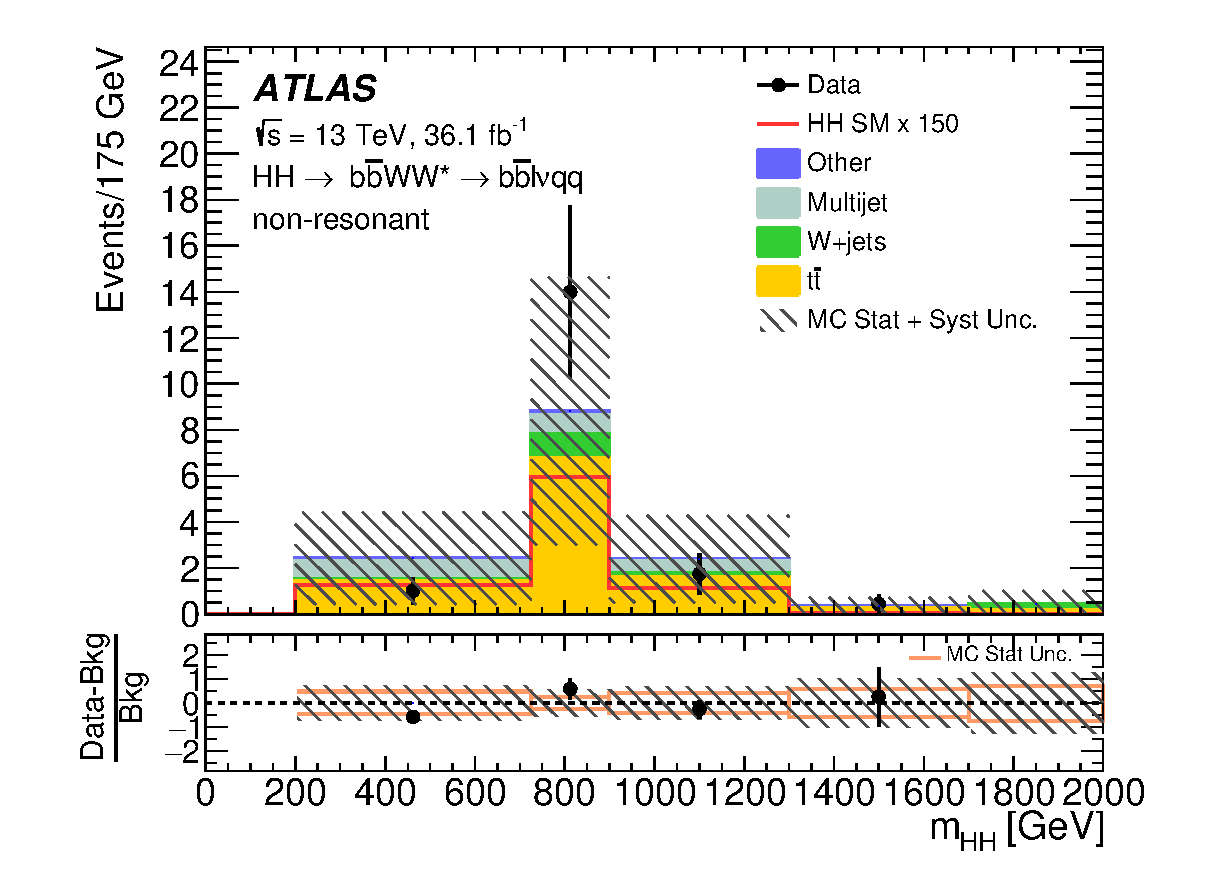
\includegraphics[width=0.9\textwidth]{figures/C_reOptNonRes_mww_bbpt210_bbpt300_wwpt250_mbb_hhMass_regionA_met25d020}\\
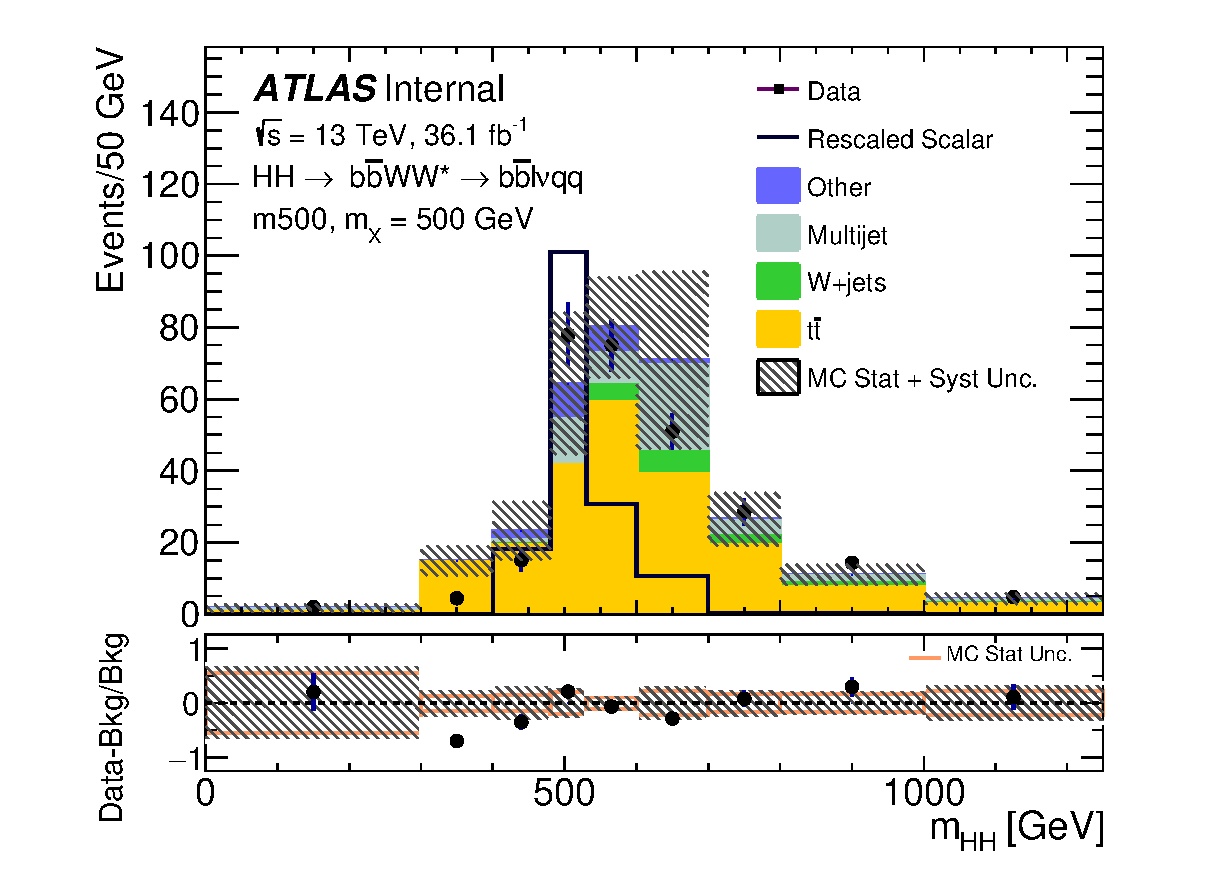
\includegraphics[width=0.9\textwidth]{figures/C_reOpt500_mww_bbpt210_wwpt150_mbb_hhMass_regionA_met25d020}
\end{center}
\end{column}
\begin{column}{0.5\textwidth}
\begin{center}
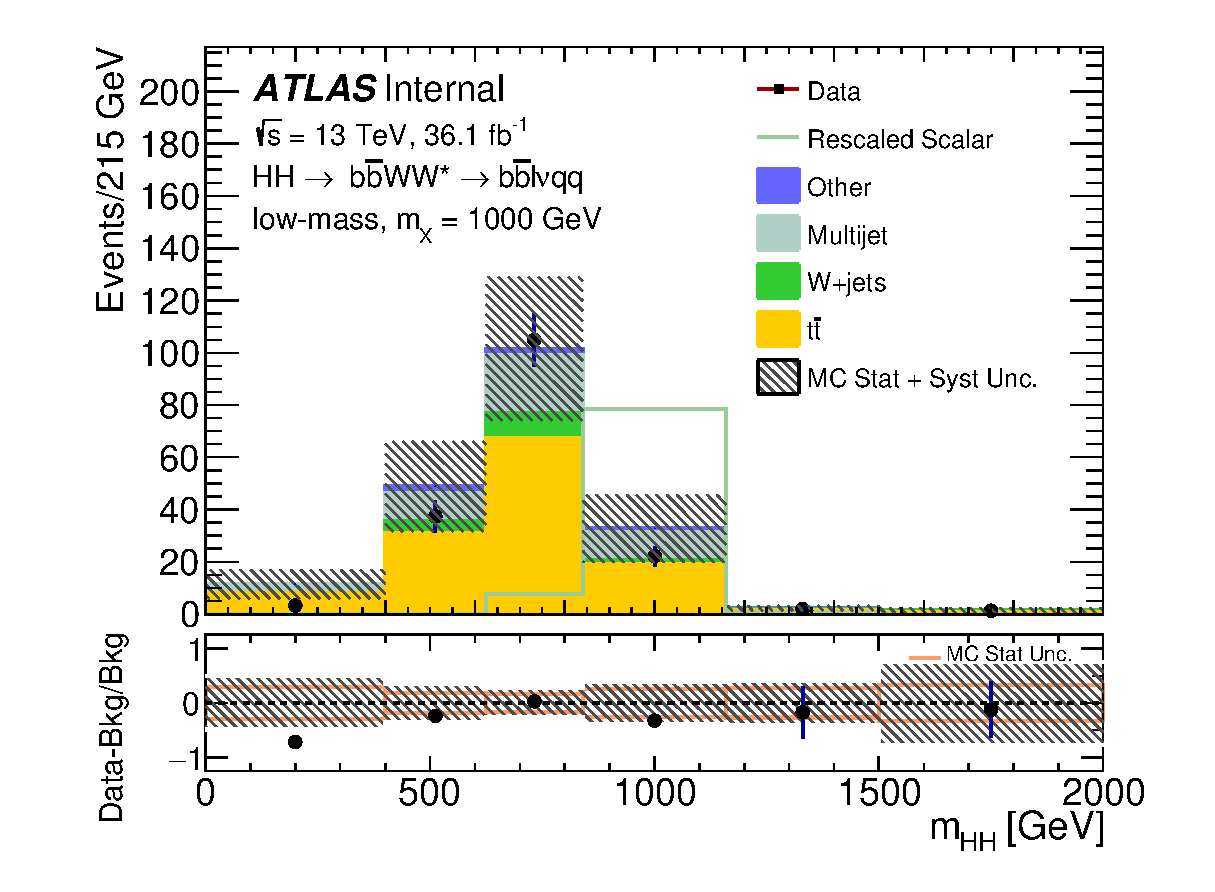
\includegraphics[width=0.9\textwidth]{figures/C_reOpt700_mww_bbpt210_wwpt250_mbb_hhMass_regionA_met25d020}\\
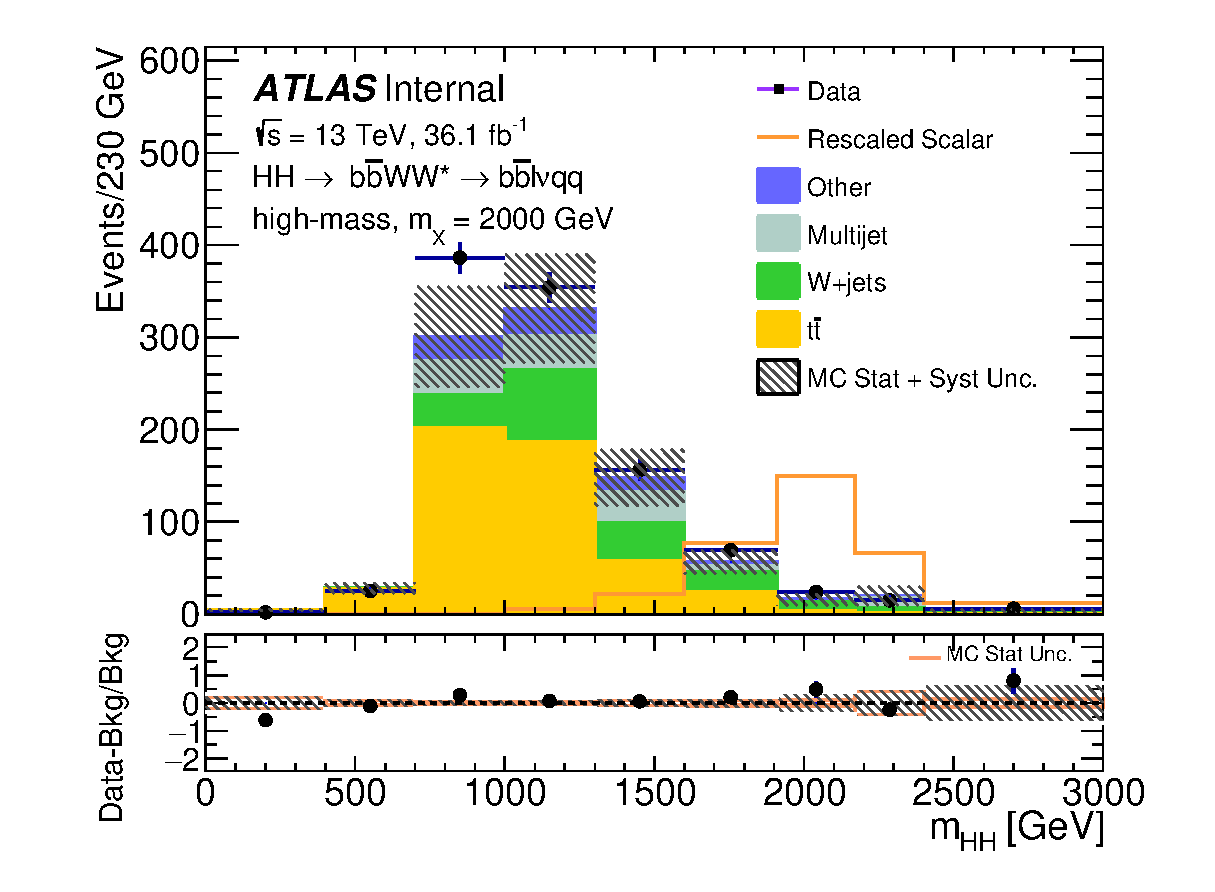
\includegraphics[width=0.9\textwidth]{figures/C_reOpt2000_bbpt350_wwpt250_drww15_mbb_hhMass_regionA_met25d020}
\end{center}
\end{column}
\end{columns}
\end{frame}

\begin{frame}
\begin{center}
\header{Boosted SR $\mathbf{m_{HH}}$}
\end{center}
\begin{center}
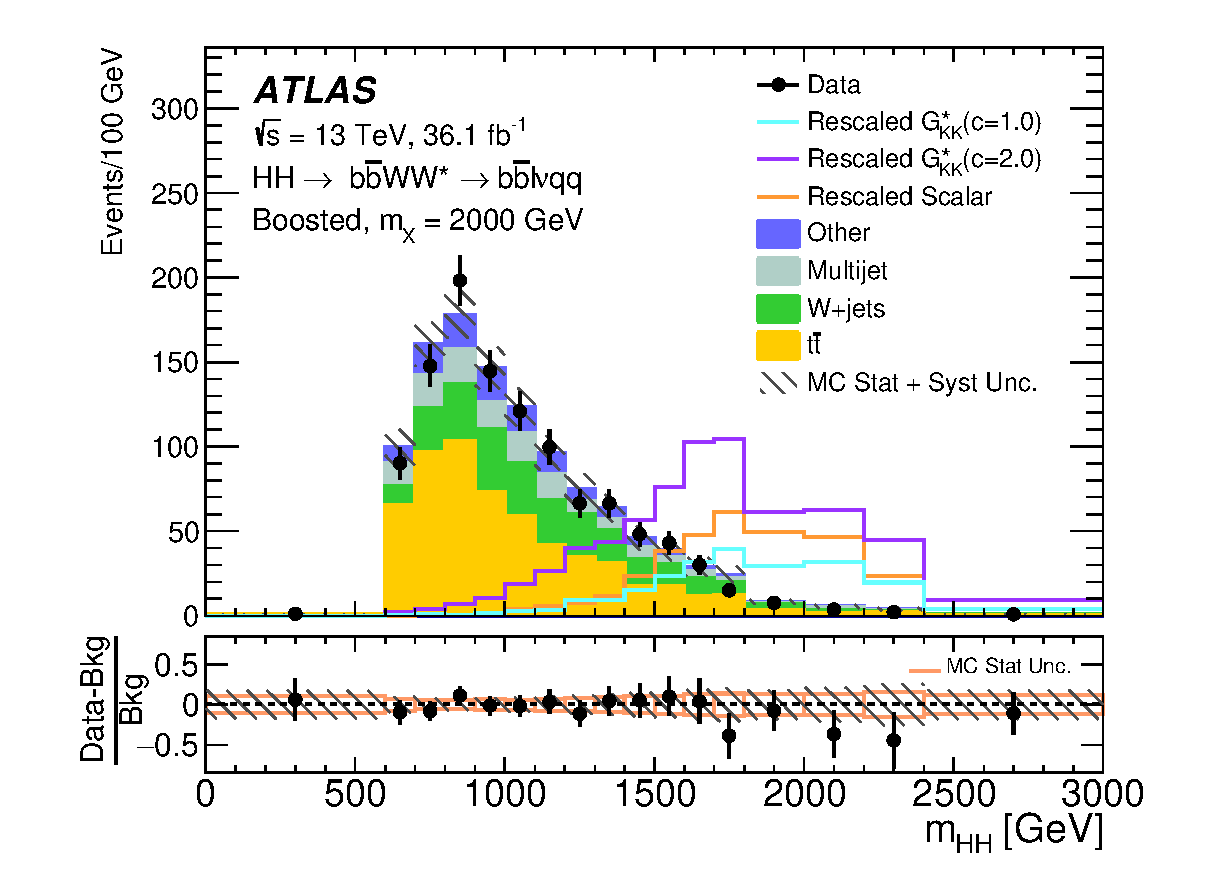
\includegraphics[width=0.8\textwidth]{figures/C_2tab_0bjet_SR_lepton_presel_met50_hhMassRebin1_postfit}
\end{center}
\end{frame}

\begin{frame}
\begin{center}
\header{Truth Study}
\end{center}
\vspace{-0.6cm}
\begin{columns}
\begin{column}{0.5\textwidth}
\begin{center}
\includegraphics[width=0.7\textwidth]{figures/drbb}\\
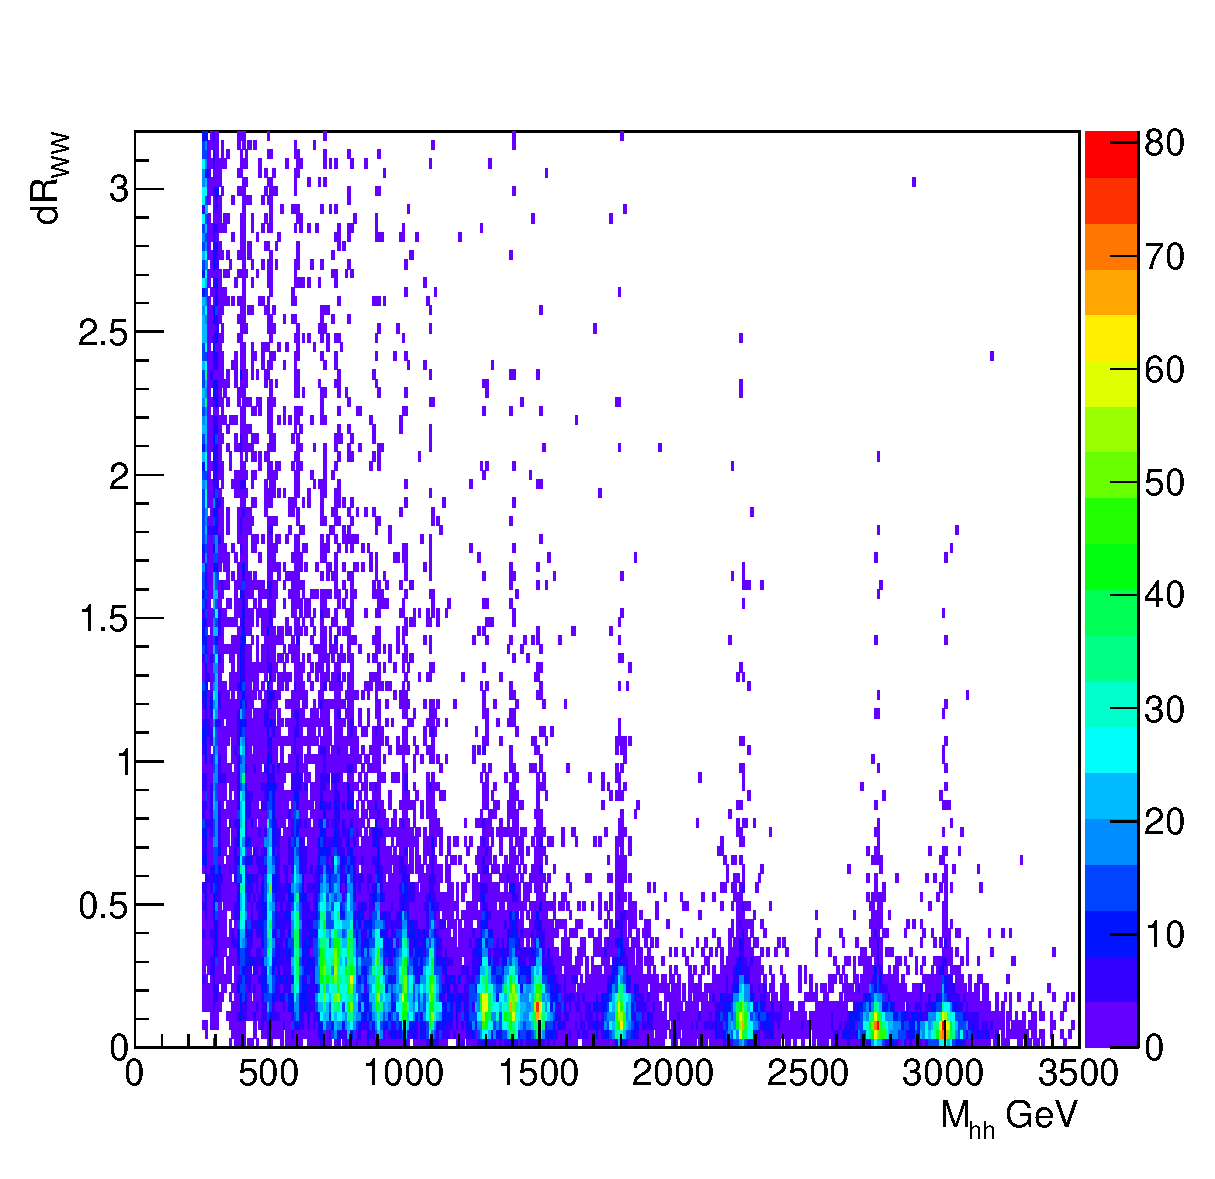
\includegraphics[width=0.7\textwidth]{figures/drWW}
\end{center}
\end{column}
\begin{column}{0.5\textwidth}
\begin{center}
\includegraphics[width=0.7\textwidth]{figures/drqq}\\
\includegraphics[width=0.7\textwidth]{figures/drminlq}
\end{center}
\end{column}
\end{columns}
\end{frame}


\begin{frame}
\begin{center}
\header{Kinematic Variable Definition}
\end{center}
\begin{center}
Neutrino reco:\\
$m_h^2 = (p^{\nu} + p^{\mathrm{large-R\ jet}})^2$\\~\\
\begin{table}
\tiny
\begin{tabular}{l|c}
\hline
\\
Lepton Channel & Alternative $p_T$ definition \\
\hline
Muon Channel & ${p_T^{'} = p_T^{\mathrm{Large-R jet}}}$\\
\hline
\\
Electron channel & ${p_T^{'} = \sqrt{(p_{x}^{\mathrm{Large-R jet}} - p_{x}^{\mathrm{electron}})^{2}+(p_{y}^{\mathrm{Large-R jet}} - p_{y}^{\mathrm{electron}})^{2}}}$
\end{tabular}
\end{table}
\end{center}
\end{frame}

\begin{frame}
\begin{center}
\header{Reconstructed Variables e-Channel}
\end{center}
\vspace{-0.5cm}
\begin{columns}
\begin{column}{0.5\textwidth}
\begin{center}
\includegraphics[width=0.7\textwidth]{figures/WHad_plots_john_withcuts/electron/hww_m_Xhh2000}\\
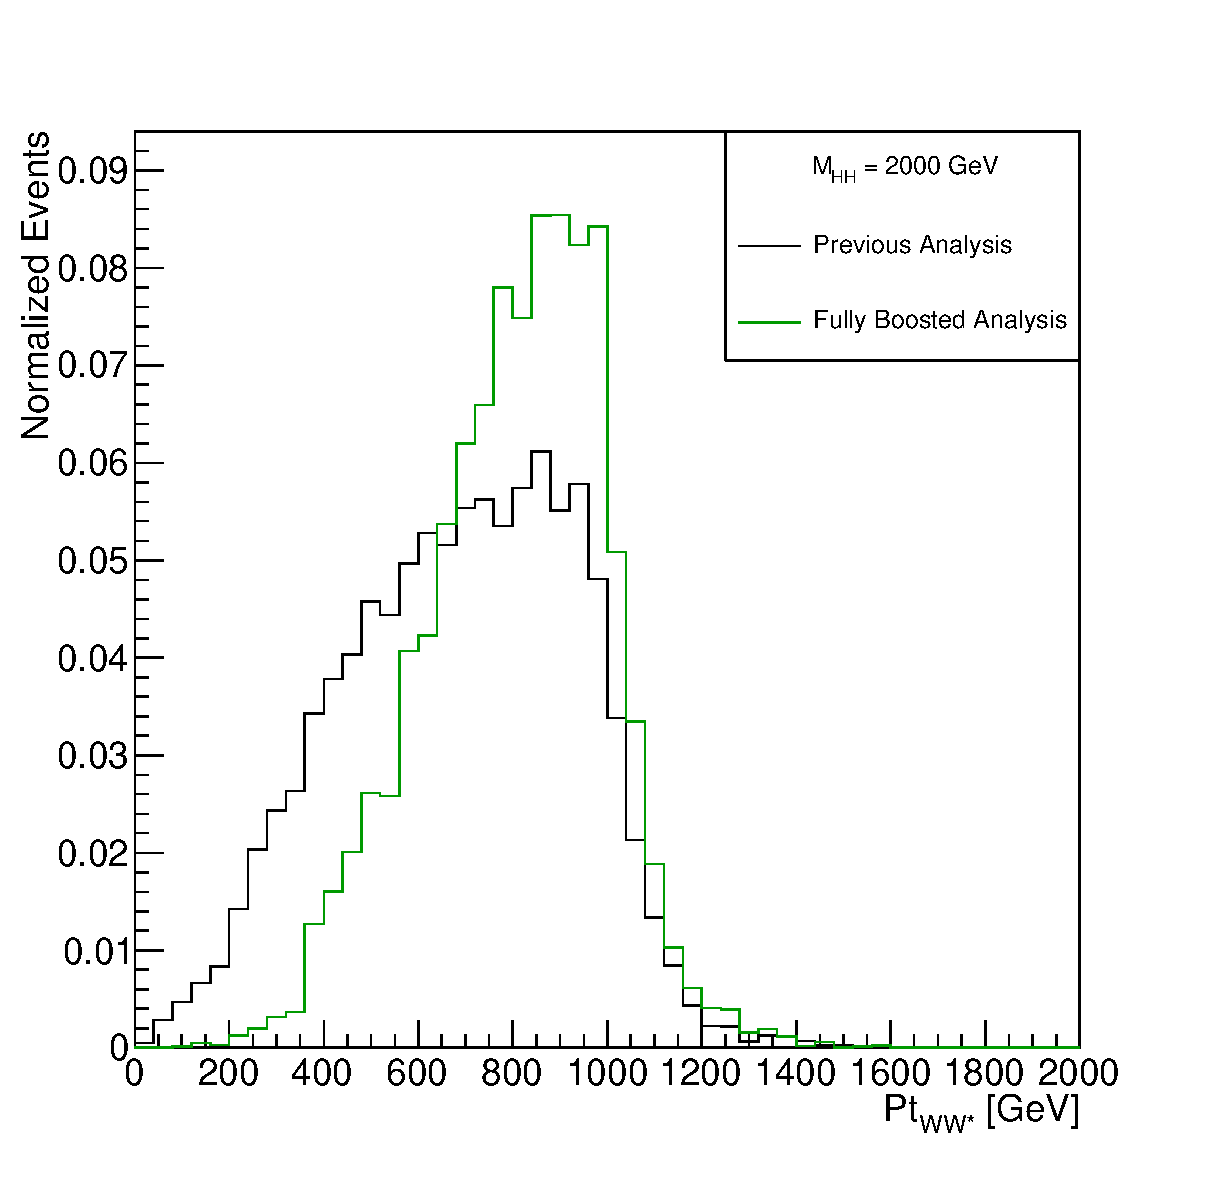
\includegraphics[width=0.7\textwidth]{figures/WHad_plots_john_withcuts/electron/hww_pt_Xhh2000}
\end{center}
\end{column}
\begin{column}{0.5\textwidth}
\begin{center}
\includegraphics[width=0.7\textwidth]{figures/WHad_plots_john_withcuts/electron/wlep_met_Xhh2000}\\
\includegraphics[width=0.7\textwidth]{figures/WHad_plots_john_withcuts/electron/hh_m_Xhh2000}
\end{center}
\end{column}
\end{columns}
\end{frame}

\begin{frame}
\begin{center}
\header{Reconstructed Variables mu-Channel}
\end{center}
\vspace{-0.5cm}
\begin{columns}
\begin{column}{0.5\textwidth}
\begin{center}
\includegraphics[width=0.7\textwidth]{figures/WHad_plots_john_withcuts/muon/hww_m_Xhh2000}\\
\includegraphics[width=0.7\textwidth]{figures/WHad_plots_john_withcuts/muon/hww_pt_Xhh2000}
\end{center}
\end{column}
\begin{column}{0.5\textwidth}
\begin{center}
\includegraphics[width=0.7\textwidth]{figures/WHad_plots_john_withcuts/muon/wlep_met_Xhh2000}\\
\includegraphics[width=0.7\textwidth]{figures/WHad_plots_john_withcuts/muon/hh_m_Xhh2000}
\end{center}
\end{column}
\end{columns}
\end{frame}

\begin{frame}
\begin{center}
\header{Fully Boosted SR}
\end{center}
\begin{table}
\begin{tabular}{l|c|c|c}
\hline
Sample        &  Yield   &  Stats Unc \\ 
\hline 
$\ttbar$    &  187.7  & $\pm$ 8.8    \\
W+Jets        &  33.7   & $\pm$ 1.9     \\
QCD           &  34.5   & $\pm$ 5.5     \\
Single-top    &  7.0   & $\pm$ 1.3     \\
Z+Jets        &  4.7    & $\pm$ 0.4        \\
Dibosons      &  3.3    & $\pm$ 0.6      \\
\hline
Prediction    &  271.0  & $\pm$ 10.7       \\
\hline
\end{tabular}
\end{table}
\end{frame}

\begin{frame}
\begin{center}
\header{Electron Reco. $\mathbf{m_{WW}}$}
\end{center}
\vspace{-0.6cm}
\begin{columns}
\begin{column}{0.5\textwidth}
\begin{center}
\color{MyPurple}{Paper Boosted Analysis}\\
\includegraphics[width=0.9\textwidth]{figures/JohnPlots_5_24/electron/hww_m/hww_m_Xhh2000sigbkg_resolved}
\end{center}
\end{column}
\begin{column}{0.5\textwidth}
\begin{center}
\color{MyPurple}{Fully-Boosted Analysis}\\
\includegraphics[width=0.9\textwidth]{figures/JohnPlots_5_24/electron/hww_m/hww_m_Xhh2000sigbkg_fatjet}
\end{center}
\end{column}
\end{columns}
\end{frame}

\begin{frame}
\begin{center}
\header{Muon Reco. $\mathbf{m_{WW}}$}
\end{center}
\vspace{-0.6cm}
\begin{columns}
\begin{column}{0.5\textwidth}
\begin{center}
\color{MyPurple}{Paper Boosted Analysis}\\
\includegraphics[width=0.9\textwidth]{figures/JohnPlots_5_24/muon/hww_m/hww_m_Xhh2000sigbkg_resolved}
\end{center}
\end{column}
\begin{column}{0.5\textwidth}
\begin{center}
\color{MyPurple}{Fully-Boosted Analysis}\\
\includegraphics[width=0.9\textwidth]{figures/JohnPlots_5_24/muon/hww_m/hww_m_Xhh2000sigbkg_fatjet}
\end{center}
\end{column}
\end{columns}
\end{frame}

\begin{frame}
\begin{center}
\header{Electron Reco. $\mathbf{m_{HH}}$}
\end{center}
\vspace{-0.6cm}
\begin{columns}
\begin{column}{0.5\textwidth}
\begin{center}
\color{MyPurple}{Paper Boosted Analysis}\\
\includegraphics[width=0.9\textwidth]{figures/JohnPlots_5_24/electron/hh_m/hh_m_Xhh2000sigbkg_resolved}
\end{center}
\end{column}
\begin{column}{0.5\textwidth}
\begin{center}
\color{MyPurple}{Fully-Boosted Analysis}\\
\includegraphics[width=0.9\textwidth]{figures/JohnPlots_5_24/electron/hh_m/hh_m_Xhh2000sigbkg_fatjet}
\end{center}
\end{column}
\end{columns}
\end{frame}

\begin{frame}
\begin{center}
\header{Muon Reco. $\mathbf{m_{HH}}$}
\end{center}
\vspace{-0.6cm}
\begin{columns}
\begin{column}{0.5\textwidth}
\begin{center}
\color{MyPurple}{Paper Boosted Analysis}\\
\includegraphics[width=0.9\textwidth]{figures/JohnPlots_5_24/muon/hh_m/hh_m_Xhh2000sigbkg_resolved}
\end{center}
\end{column}
\begin{column}{0.5\textwidth}
\begin{center}
\color{MyPurple}{Fully-Boosted Analysis}\\
\includegraphics[width=0.9\textwidth]{figures/JohnPlots_5_24/muon/hh_m/hh_m_Xhh2000sigbkg_fatjet}
\end{center}
\end{column}
\end{columns}
\end{frame}

\begin{frame}
\begin{center}
\header{Fully Boosted Systematics Unc.}
\end{center}
\tiny
\begin{table}[p]
\begin{center}
\begin{tabular}{c|c}
\hline \hline
Uncertainty & Up/Down \\
\hline \hline
SysFT\_EFF\_Eigen\_Light\_0\_AntiKt2PV0TrackJets\_\_1down & -12.9/12.5 \\
SysFT\_EFF\_Eigen\_C\_0\_AntiKt2PV0TrackJets\_\_1down & -12.6/12.1 \\
SysFT\_EFF\_Eigen\_C\_0\_AntiKt2PV0TrackJets\_\_1up & 11.3/-11.9 \\
SysFT\_EFF\_Eigen\_Light\_0\_AntiKt2PV0TrackJets\_\_1up & 11.3/-11.9 \\
SysFATJET\_Medium\_JET\_Comb\_Baseline\_Kin\_\_1up & -6.47/5.95 \\
SysFATJET\_Medium\_JET\_Comb\_Baseline\_Kin\_\_1down & 5.83/-6.43 \\
SysFT\_EFF\_Eigen\_B\_0\_AntiKt2PV0TrackJets\_\_1down & -3.49/2.97 \\
SysFT\_EFF\_Eigen\_B\_1\_AntiKt2PV0TrackJets\_\_1down & -3.32/2.8 \\
SysFT\_EFF\_Eigen\_C\_1\_AntiKt2PV0TrackJets\_\_1down & -2.97/2.45 \\
SysFT\_EFF\_Eigen\_B\_0\_AntiKt2PV0TrackJets\_\_1up & 2.39/-2.94 \\
SysFT\_EFF\_Eigen\_B\_1\_AntiKt2PV0TrackJets\_\_1up & 2.23/-2.78 \\
SysFT\_EFF\_Eigen\_C\_1\_AntiKt2PV0TrackJets\_\_1up & 1.9/-2.45 \\
SysFATJET\_Medium\_JET\_Comb\_Tracking\_Kin\_\_1down & 1.77/-2.38 \\
SysFATJET\_Medium\_JET\_Comb\_Tracking\_Kin\_\_1up & -2.2/1.68 \\
SysFT\_EFF\_extrapolation\_AntiKt2PV0TrackJets\_\_1up & -2.07/1.59 \\
SysFATJET\_JMR\_\_1up & 1.41/-1.97 \\
SysFT\_EFF\_extrapolation\_from\_charm\_AntiKt2PV0TrackJets\_\_1up & -1.62/1.1 \\
SysFT\_EFF\_extrapolation\_AntiKt2PV0TrackJets\_\_1down & 0.963/-1.54 \\
SysPRW\_DATASF\_\_1down & -1.47/0.94 \\
SysJET\_SR1\_JET\_GroupedNP\_1\_\_1down & 0.764/-1.33 \\
SysJET\_SR1\_JET\_GroupedNP\_1\_\_1up & -1.2/0.678 \\
SysFATJET\_JER\_\_1up & 0.574/-1.16 \\
SysFT\_EFF\_Eigen\_Light\_1\_AntiKt2PV0TrackJets\_\_1up & -1.12/0.576 \\
SysFT\_EFF\_extrapolation\_from\_charm\_AntiKt2PV0TrackJets\_\_1down & 0.553/-1.1 \\
SysFATJET\_Medium\_JET\_Comb\_TotalStat\_Kin\_\_1down & -1.03/0.498 \\
Total Up & 27.2\\
Total Do & 27.7\\
\hline \hline
\end{tabular}
\end{center}
\end{table}
\end{frame}


\backupend
\end{document}


